%----------------------------------------------------------------------------------------
%	TITLE PAGE
%----------------------------------------------------------------------------------------

\begingroup
\thispagestyle{empty}
\begin{tikzpicture}[remember picture,overlay]
  \coordinate [below=12cm] (midpoint) at (current page.north);
  \node at (current page.north west)
  {\begin{tikzpicture}[remember picture,overlay]
      \node[anchor=north west,inner sep=0pt] at (0,0) {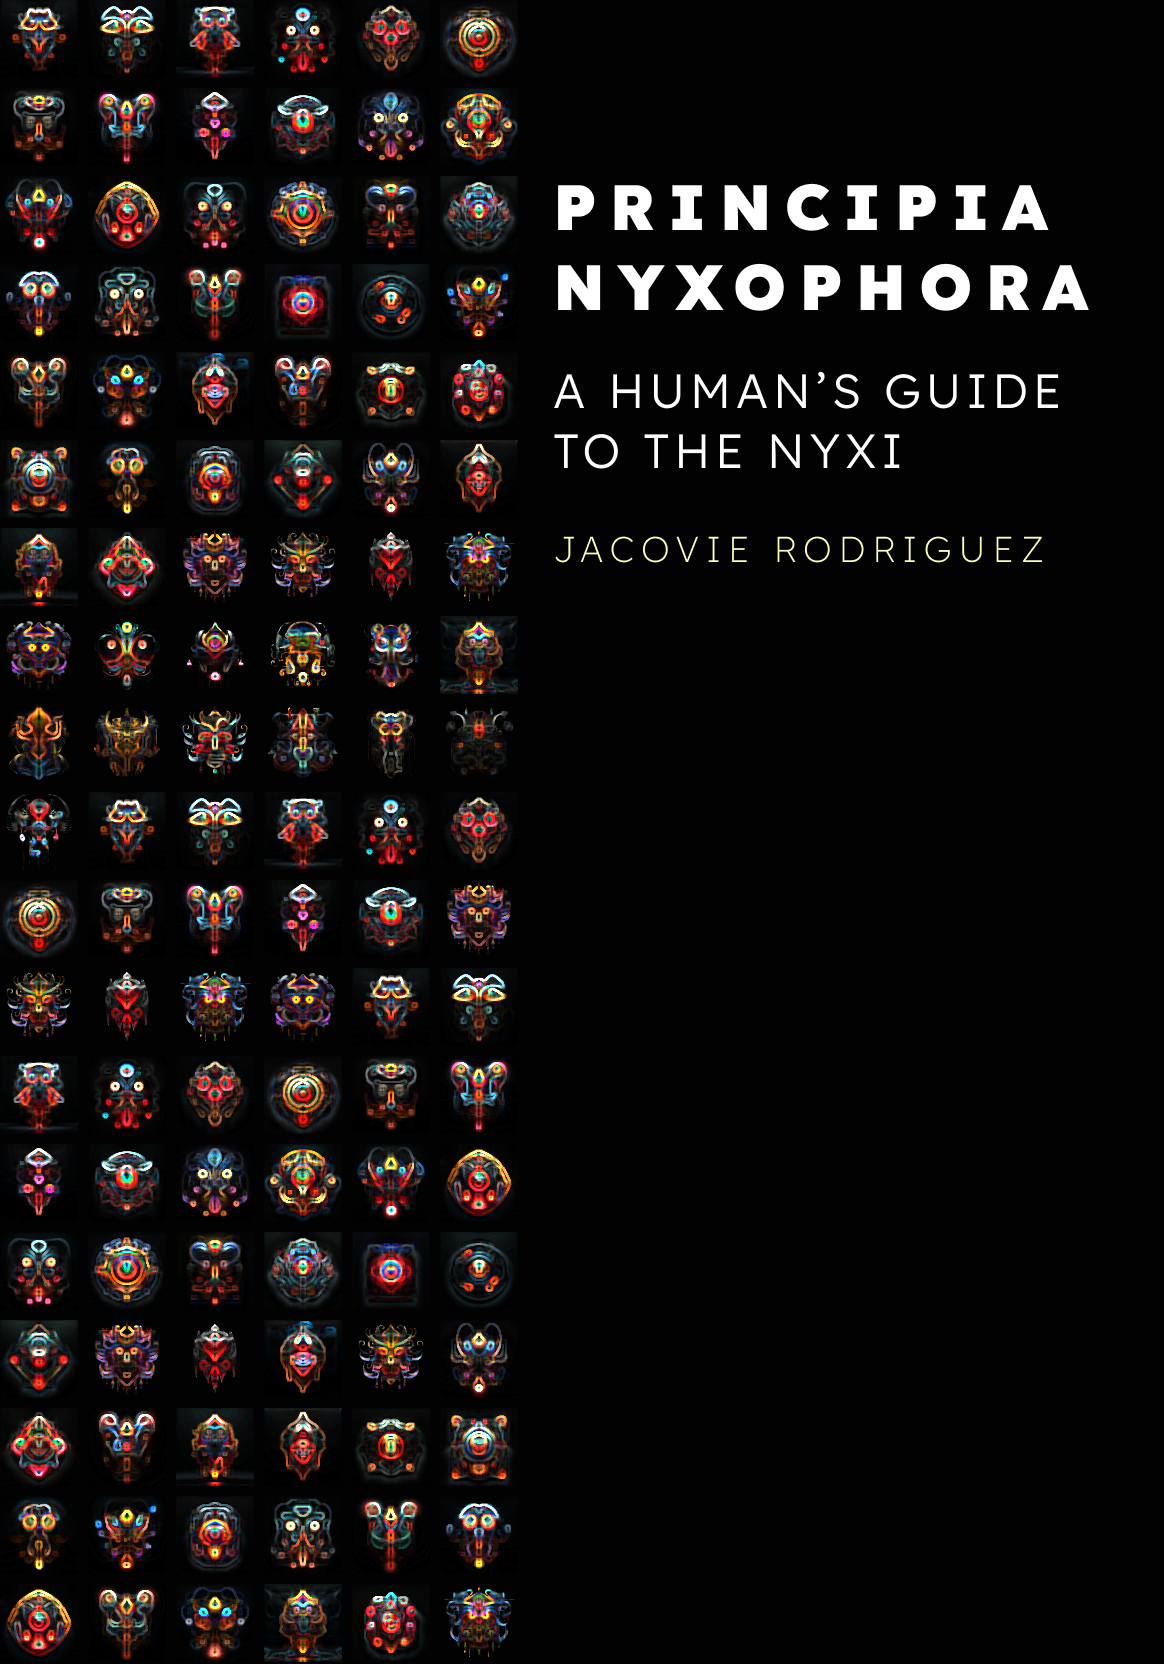
\includegraphics[width=\paperwidth]{images/NyxCoverV2.png}}; % Background image
    \end{tikzpicture}};
\end{tikzpicture}
\vfill
\endgroup

%----------------------------------------------------------------------------------------
%	COPYRIGHT PAGE
%----------------------------------------------------------------------------------------

\newpage
~\vfill
\thispagestyle{empty}

\noindent Copyright \copyright\ 2023 Jacovie Rodriguez\\ % Copyright notice

\noindent \textsc{Published by Publisher}\\ % Publisher

\noindent \textsc{book-website.com}\\ % URL

\noindent Licensed under the Creative Commons Attribution-NonCommercial 3.0 Unported License (the ``License''). You may not use this file except in compliance with the License. You may obtain a copy of the License at \url{http://creativecommons.org/licenses/by-nc/3.0}. Unless required by applicable law or agreed to in writing, software distributed under the License is distributed on an \textsc{``as is'' basis, without warranties or conditions of any kind}, either express or implied. See the License for the specific language governing permissions and limitations under the License.\\ % License information

\noindent \textit{First printing, August 2023} % Printing/edition date

%----------------------------------------------------------------------------------------
%	TABLE OF CONTENTS
%----------------------------------------------------------------------------------------

%\usechapterimagefalse % If you don't want to include a chapter image, use this to toggle images off - it can be enabled later with \usechapterimagetrue

\chapterimage{chapter0_header.png} % Table of contents heading image

\pagestyle{empty} % No headers

\tableofcontents % Print the table of contents itself

\clearpage % Forces the first chapter to start on an odd page so it's on the right

If you're reading this, then thanks so much for taking the time to enjoy my
inner universe! This "explorative textbook" is a tool to compile all the
details of the worldbuilding I've been doing on the side. The main concept was
to think through creating a language that was truly alien, not based on human
physiology whatsoever, and then expanding the history and culture of these
alien beings to build their world and also help inspire the lexicon of their
language.

The rest of this book is written from the perspective of humanity in this
world, circa the year 4242. While I do have a goal of some level of scientific
realism in this world, I also stay open to bend into fiction if it offers a
particularly interesting development. After all, if this in the far future, I
anticipate we've had many advances in our scientific knowledge.

In some cases I might offer some explanatory footnotes, but otherwise this is
the last you'll be hearing from "me". As I see you off into the world of the
Nyxi, I hope you enjoy your adventure! \\[48pt]
\hrule

\begin{center}
  \textit{Dedicated to Andrew, from Jacovie and Neb}
\end{center}

\pagestyle{fancy} % Print headers again 